\usetikzlibrary{positioning,shapes,shadows,arrows}
\tikzstyle{conf}=[rectangle, draw=black, rounded corners, fill=gray!50, drop shadow,
        text centered, anchor=north, text=white, text width=3cm,top color=gray, bottom color=gray!40]
\tikzstyle{sp-cont}=[rectangle, draw=black, rounded corners, fill=blue!50, drop shadow,
        text centered, anchor=north, text=white, text width=3cm,top color=blue!60, bottom color=blue!20]
\tikzstyle{sim}=[rectangle, draw=black, rounded corners, fill=orange, drop shadow,
        text centered, anchor=north, text=white, text width=3cm,top color=orange, bottom color=orange!40]
\tikzstyle{sim2}=[rectangle, draw=black, fill=white,
        text centered, anchor=north, text=white, text width=3cm]
        
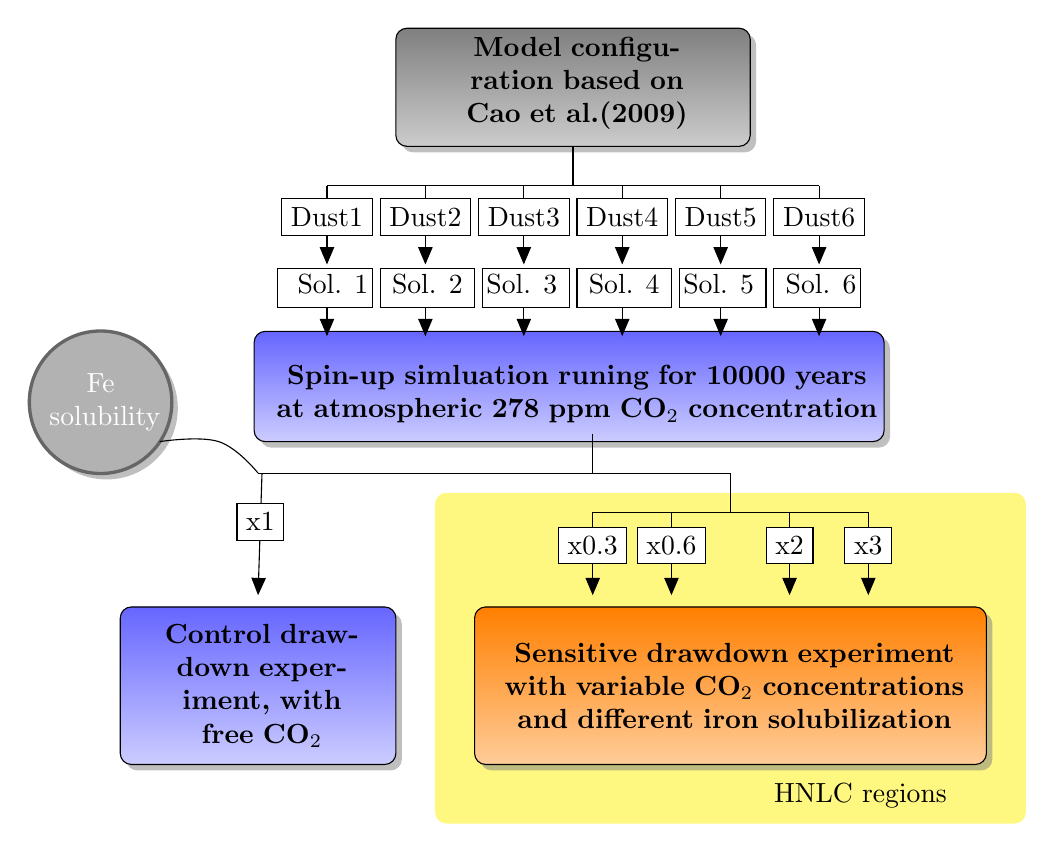
\begin{tikzpicture}
\draw[conf]  (-2.5,2.25) rectangle (2,0.75);
\draw[sp-cont] (-4.3,-1.6) rectangle (3.7,-3);
\draw[sp-cont] (-6,-5.1) rectangle (-2.5,-7.1);
\draw[rounded corners,fill=yellow!50,draw=none]  (-2,-3.65) rectangle (5.5,-7.85);
\draw[sim] (-1.5,-5.1) rectangle (5,-7.1);
\node[text width=4cm,text centered] at (-0.2,1.55) {\textbf{Model configuration based on Cao et al.(2009)}};
\draw (-0.25,0.75) node (v1) {} -- (-0.25,0.25) node (v2) {} -- (2.875,0.25) node (v4) {};
\draw (v1) -- (-0.25,0.25) -- (-3.375,0.25) node (v3) {};
\draw[-triangle 45] (-3.375,0.25) -- node [ style={pos=0.4},draw=black,fill=white,scale=1] {Dust1} (-3.375,-0.75);
\draw[sim2] (-4,-0.8) rectangle (-2.8,-1.3);
\draw[sim2] (-1.5,-0.8) rectangle (-2.7,-1.3);
\draw[sim2] (-0.29,-0.8) rectangle (-1.4,-1.3);
\draw[sim2] (1,-0.8) rectangle (-0.2,-1.3);
\draw[sim2] (2.2,-0.8) rectangle (1.1,-1.3);
\draw[sim2] (3.4,-0.8) rectangle (2.3,-1.3);
\draw[sim2] (-1.5,-0.8) rectangle (-2.7,-1.3);
\draw[-triangle 45] (2.875,0.25) -- node [ style={pos=0.4},draw=black,fill=white,scale=1] {Dust6}(2.875,-0.75);
\draw[-triangle 45] (-2.125,0.25) -- node [ style={pos=0.4},draw=black,fill=white,scale=1] {Dust2}(-2.125,-0.75);
\draw[-triangle 45] (-0.875,0.25) -- node [ style={pos=0.4},draw=black,fill=white,scale=1] {Dust3}(-0.875,-0.75);
\draw[-triangle 45] (1.625,0.25) -- node [ style={pos=0.4},draw=black,fill=white,scale=1] {Dust5}(1.625,-0.75);
\draw[-triangle 45] (0.375,0.25) -- node [ style={pos=0.4},draw=black,fill=white,scale=1] {Dust4}(0.375,-0.75);
\draw (0,-2.9) node (v5) {} -- (0,-3.4) node (v6) {} -- (1.75,-3.4) node (v7) {};
\draw (v5) -- (0,-3.4) -- (-4.25,-3.4) node (v11) {};
\draw (1.75,-3.4) -- (1.75,-3.9) node (v8) {} -- (3.5,-3.9) node (v10) {};
\draw (v7) -- (1.75,-3.9) -- (0,-3.9) node (v9) {};
\draw[-triangle 45] (0,-3.9) -- node [ style={pos=0.4},draw=black,fill=white,scale=1] {x0.3}(0,-4.95);
\draw[-triangle 45] (3.5,-3.9) -- node [ style={pos=0.4},draw=black,fill=white,scale=1] {x3}(3.5,-4.95);
\draw[-triangle 45] (1,-3.9) -- node [ style={pos=0.4},draw=black,fill=white,scale=1] {x0.6}(1,-4.95);
\draw[-triangle 45] (2.5,-3.9) -- node [ style={pos=0.4},draw=black,fill=white,scale=1] {x2}(2.5,-4.95);
\draw[-triangle 45] (-4.2,-3.4) -- node [ style={pos=0.4},draw=black,fill=white,scale=1] {x1}(-4.25,-4.95);
\node[text width=8cm,text centered] at (-0.2,-2.4) {\textbf{Spin-up simluation  runing for 10000 years at atmospheric 278 ppm CO$_2$ concentration}};
\node[text width=3cm,text centered] at (-4.2,-6.1) {\textbf{Control drawdown experiment, with free CO$_2$}};
\node at (3.4,-7.5) {HNLC regions};
\node[text width=6cm,text centered] at (1.8,-6.1) {\textbf{Sensitive drawdown experiment with variable CO$_2$ concentrations and different iron solubilization}};
\node at (1.8,-6.1) {};
\node at (1.8,-6.1) {};
\node at (1.8,-6.1) {};
\node at (1.8,-6.1) {};
\draw[-triangle 45] (-3.375,-1.3) -- (-3.375,-1.66);
\draw[-triangle 45] (-2.125,-1.3) -- (-2.125,-1.66);
\draw[-triangle 45] (-0.875,-1.3) -- (-0.875,-1.66);
\draw[-triangle 45] (0.375,-1.3) -- (0.375,-1.66);
\draw[-triangle 45] (1.625,-1.3) -- (1.625,-1.66);
\draw[-triangle 45] (2.875,-1.3) -- (2.875,-1.66);
\node at (-3.3,-1) {Sol. 1};
\node at (-2.1,-1) {Sol. 2};
\node at (-0.9,-1) {Sol. 3};
\node at (0.4,-1) {Sol. 4};
\node at (1.6,-1) {Sol. 5};
\node at (2.9,-1) {Sol. 6};
\node[circle,draw,color=black!60,text=white,fill=gray!60, very thick,drop shadow,text width=1.3cm,text centered] (c) at (-6.25,-2.5) {Fe\\ solubility};

\draw  plot[smooth, tension=.7] coordinates {(c)};
\draw  plot[smooth, tension=.7] coordinates {(-5.5,-3) (-4.75,-3) (v11)};
\end{tikzpicture}